\documentclass{article}
\usepackage[utf8]{inputenc}
\usepackage{amsmath}
\usepackage{amssymb}
\usepackage{amsfonts}
\usepackage{amssymb}
\usepackage{minted}
\usepackage{graphicx}
\graphicspath{ {img/} }
\usepackage{titlesec}
\usepackage[a4paper,margin=1in,footskip=0.25in]{geometry}
\usepackage{fancyhdr}
\pagestyle{fancy}
%basic page layout

%draw finite state machine
\usepackage{tikz}
\usetikzlibrary{arrows,automata}
\newcommand{\hwnumber}{2}
\newcommand{\Lcvy}{\mathcal{L}}
%header and footer settings
\lhead{Gen IMS II Homework \hwnumber}
\chead{Yiping Deng}
\rhead{\today}

\titlelabel{\thetitle\enspace}

\begin{document}
\title{Gen IMS II Homework \hwnumber}
\author{Yiping Deng}
\maketitle
\thispagestyle{fancy}
\section*{Task 1}
\subsection*{a)}
Using physics, we have
\begin{align}
    V_{L} &= L \frac{dI}{dt} \\
    V_{R} &= IR \\
    V_{L} + V_{R} &= V_{S}
\end{align}
Substitute (1), (2) into (3), we get the ODE
\begin{align}
    L \frac{dI}{dt} + IR &= V_{S}
\end{align}
\subsection*{b)}
Since it is a seperable ODE, we can solve it using seperation
of variable.
\begin{align}
    \implies (IR - V_{S})dt &= -L dI \\
    \implies dt &= -L \frac{dI}{IR - V_{S}} \\
    \implies t + C &= -\frac{L}{R} ln(IR - V_{S}) \\
    \implies ln(IR-V_{S}) &= -\frac{R}{L} t + C \\
    \implies IR - V_{S} &= C e^{-\frac{R}{L} t} \\
    \implies I &= \frac{V_{S}}{R} + C e^{-\frac{R}{L} t}
\end{align}
Note that C is the constant derived from integration. \\
Now we can plug in the initial value that $I(0) = I_{ini}$
\begin{align}
    I_{ini} &= \frac{V_{S}}{R} + C \implies \\
    C &= I_{ini} - \frac{V_{S}}{R}
\end{align}
Thus, this give us the solution for the differential equation.
\begin{align}
    I(t) &= \frac{V_{S}}{R} + \frac{I_{ini} R - V_{S}}{R} e^{-\frac{R}{L} t}
\end{align}
\subsection*{c)}
Take Laplace transform on both side of (4)
\begin{align}
    \Lcvy(L \frac{dI}{dt} + IR) &= \Lcvy(V_{S})
\end{align}
Using the linearity, we can get
\begin{align}
    L \Lcvy(I') + R \Lcvy(I) &= V_{S} \Lcvy(1)
\end{align}
We use $I^*$ to represent function in frequency domain.
\begin{align}
    L(sI^*(s) - I(0)) + RI^*(s) &= V_{S} \frac{1}{s} \\
    I(0) &= I_{ini} \implies \\
    L(sI^*(s) - I_{ini}) + RI^*(s) &= V_{S} \frac{1}{s} \\
    \text{With simplification: }
    (s^2 L + sR) I^*(s) &= V_{S} + I_{ini} R \\
    I^*(s) &= \frac{V_{S} + I_{ini} R}{s^2 L + s R}
\end{align}
We factorize the right-hand side of (20), and apply inverse Laplace transform
\begin{align}
    I^*(s) &= \frac{V_{S}}{R} \frac{1}{s} + \frac{I_{ini} R - V_{S}}{R} \frac{1}{s + \frac{R}{L}}
\end{align}
Apply Inverse Laplace Transform
\begin{align}
    I(t) &= \Lcvy(I^*(s)) = \frac{V_{S}}{R} + \frac{I_{ini} R - V_{S}}{R} e^{-\frac{R}{L} t}
\end{align}
\subsection*{c)}
To evaluate $ t = 0.000002$, with plot $\Delta x = 0.000002 / 5 $, $\Delta x = 0.000002 / 10 $,
$\Delta x = 0.000002 / 20 $
\inputminted{Python}{plot.py}
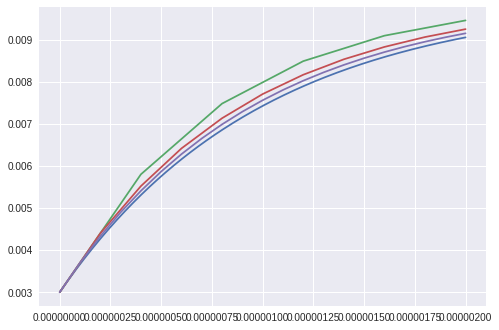
\includegraphics{plot.png}
\inputminted{Python}{plot.dt}
As you can see in the picture, the finer the $\Delta x$, the closer
it approaches to the solution. This iteration scheme converges uniformly to the solution function.
\end{document}
